\documentclass[11pt, a4paper]{article} % setsfont size and layout

%% required packages %%

\usepackage[margin=2.5cm]{geometry} % margins
\usepackage[english]{babel} % language (replace with german or ngerman for german texts)
\usepackage[utf8]{inputenc} % Umlaute
\usepackage{amsmath}		% math formulas
\usepackage{graphicx}		% graphics
\usepackage{fancyhdr}		% header and footer on every page
\usepackage{setspace}		% line space (e.g. \singlespacing, \onehalfspacing or \doublespacing)
\usepackage{xcolor}
\usepackage{pdflscape}
\usepackage{rotating}
\usepackage[boxruled, lined, vlined]{algorithm2e}
\SetKwFor{For}{for (}{) $\lbrace$}{$\rbrace$}
\usepackage{bm}
\usepackage{caption}
\usepackage{subcaption}
\usepackage{float}
\usepackage{multicol}

\begin{document}
	
%% Some more settings %%
	
\setlength{\parindent}{0pt} % first line in paragraph will not be indented
\onehalfspacing				% 1.5 line spacing
%\thispagestyle{empty}		% no header and page number on first page


%% Header on first page with course information etc. %%
\begin{tabular}{p{15.5cm}}
	{\large \textbf{Inrobin}} \\
	Gareth W. Peters  \\ 
	Dorota Toczydłowska\\
	Marta Campi\\
	\hline
	\\
\end{tabular}

\vspace*{0.3cm}				% vertical space between header on top of the page and main heading


\begin{center}
	{\LARGE \textbf{Experiment two speech signals}}
	\vspace{2mm}	
\end{center} 

\section*{Frequency bands location}
Set the notation of this experiment as follows:

$\Omega$ is the set of $M_{true}$ vectors of parameters where each vector is $J$ dimensional \\
$\Omega = \Big\{ \Psi^1, \ldots, \Psi^{M_{true}} \Big\}$\\
Let $\Psi^{j} = [\Psi^{j}_1, \ldots, \Psi^{j}_J]$ which is the $j$th element of $\Omega$ set\\
$\Psi^j_h$ is $h$th element of $\Psi^{j}$\\
$k(\cdot, \cdot;\Psi)$ a kernel function from parameterized by the parameter $\Psi$,  $k: \mathcal{R} \times \mathcal{R} \rightarrow \mathcal{R}$\\ 
Let $\mathbf{t}$ be a $1\times N$ vector of real numbers\\
$\mathbf{K} = k(\mathbf{t}, \mathbf{t};\Psi = \Psi)$\\
$j \in \Big\{ 1, \cdots, M_{true} \Big\}$, $m \in \Big\{ 1, \cdots, M \Big\}$, $h \in \Big\{1, \ldots, J \Big\}$\\ %maybe change notation
$n_{j,m}$ number of IMFs

\hfill

\begin{algorithm}[H]


\label{algo_exp1}
\caption{Algorithm}

\BlankLine
\addtolength\linewidth{-12ex}

\KwIn{Discrete speech signals}
%\KwOut{CKTA between $\mathbf{S}_{N \times N}^{(m)}$ and Kernel Gram Matrix $\mathbf{K}_{(test,i)}$ }

\begin{enumerate}

%\item Evaluate each Gram Matrix $\mathbf{K}^{(j)}_h = k(\mathbf{t},\mathbf{t}; \Psi^{(j)}_h)$ parametrized by the $j$th parameter from $\Omega$. There are $J$ Gram Matrices since $h = 1, \dots, J$ \\

%\item Simulate $\mathbf{y}_{j,h}^{(m)} \sim \mathcal{N}(0, \mathbf{K}^{(j)}_h)$ an N dimensional vector for each Gram Matrix $\mathbf{K}^{(j)}_h$, therefore we have $J$ one dimensional vectors of length $N$.\\

%\item Compute $ \mathbf{x}^{(m)}_j = \sum_{h=1}^{J} \mathbf{y}_{j,h}^{(m)} $

\item Fit a spline through each $\mathbf{x}_j^{(m)}$ denoted as $\hat{\mathbf{x}}_j^{(m)}$.

\item Apply the EMD to $ \hat{\mathbf{x}}_j^{(m)}$ to get the IMFs decomposition and collect all the IMFs generated up to the stopping criterion chosen denoted as $\bm{\gamma}^{(m)}_{j,1}, \bm{\gamma}_{j,2}^{(m)}, \dots, \bm{\gamma}_{j,v_{j,m}}^{(m)}$. For each $j$ and for each $m$ we might have different number of IMFs denote by $v_{j,m}$.

\item Compute the Instantaneous Frequency of each IMF denoted as $\bm{f}^{(m)}_{j,1}, \bm{f}_{j,2}^{(m)}, \dots, \bm{f}_{j,v_{j,m}}^{(m)}$.
\item Compare the frequencies with Spectral Component of the kernels


\end{enumerate}

\end{algorithm}


\newpage




\begin{landscape}

\begin{figure}
\begin{subfigure}{0.8\textwidth}
  \centering
  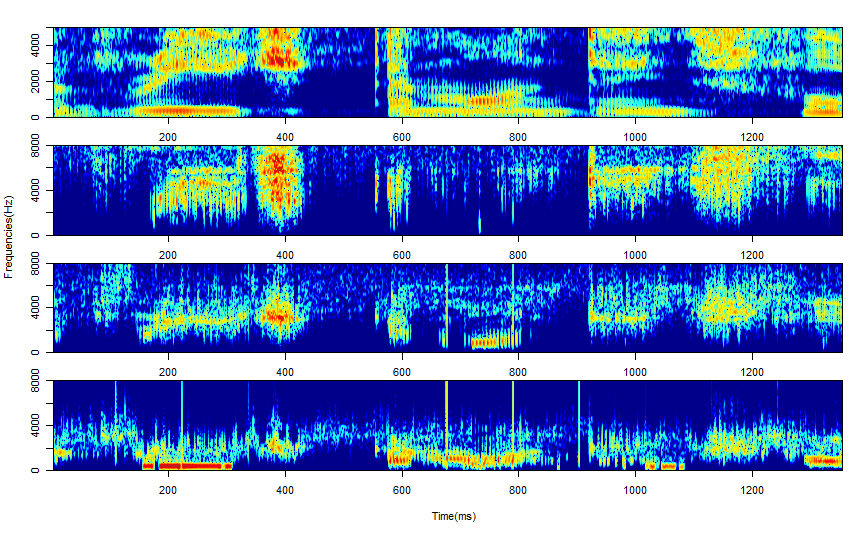
\includegraphics[width=\linewidth]{spectro_speak1.png}
%  \caption{1a}
  \label{fig:sfig1}
\end{subfigure}%
\begin{subfigure}{0.8\textwidth}
  \centering
  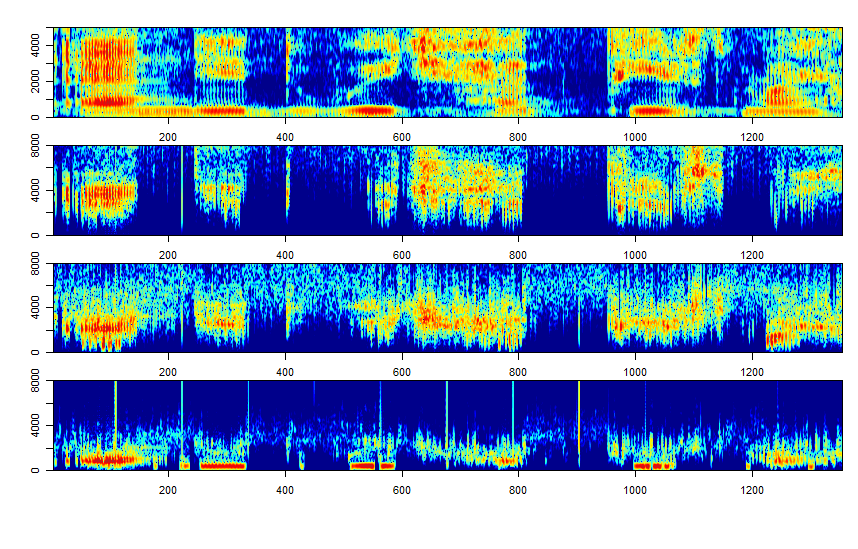
\includegraphics[width=\linewidth]{spectro_speak1_bis.png}
%  \caption{1b}
  \label{fig:sfig2}
\end{subfigure}\\
\begin{subfigure}{0.8\textwidth}
  \centering
  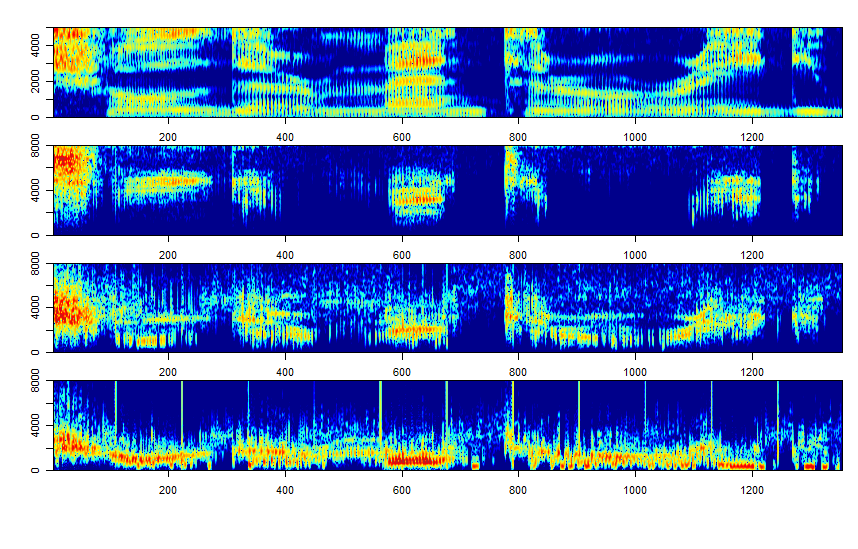
\includegraphics[width=\linewidth]{spectro_speak1_tris.png}
%  \caption{1b}
  \label{fig:sfig2}
\end{subfigure}
\label{fig1}
\caption{Spectrograms of three sentences for speaker 1 (female voice). From the top: the original signal, IMF1, IMF2 and IMF3 respectively.}
\end{figure}
\end{landscape}


\begin{landscape}
\begin{figure}
\begin{subfigure}{0.8\textwidth}
  \centering
  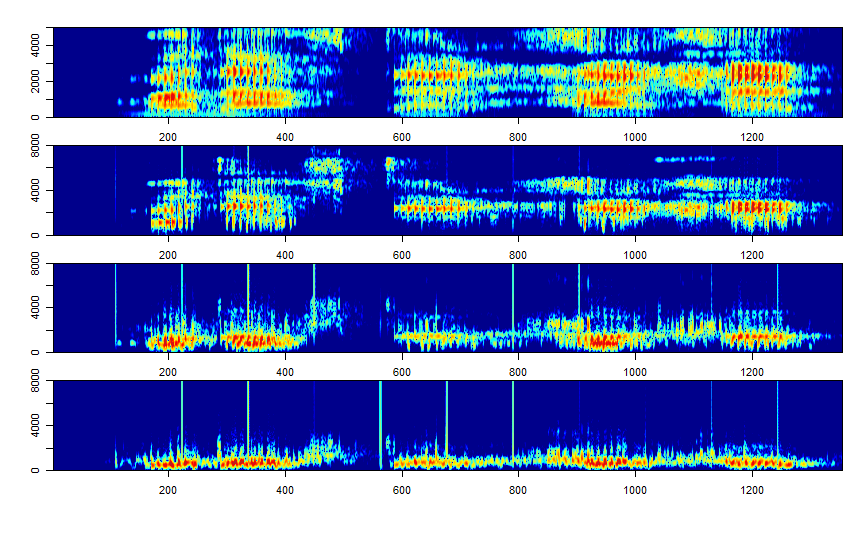
\includegraphics[width=\linewidth]{spectro_speak3.png}
%  \caption{1a}
  \label{fig:sfig1}
\end{subfigure}%
\begin{subfigure}{0.8\textwidth}
  \centering
  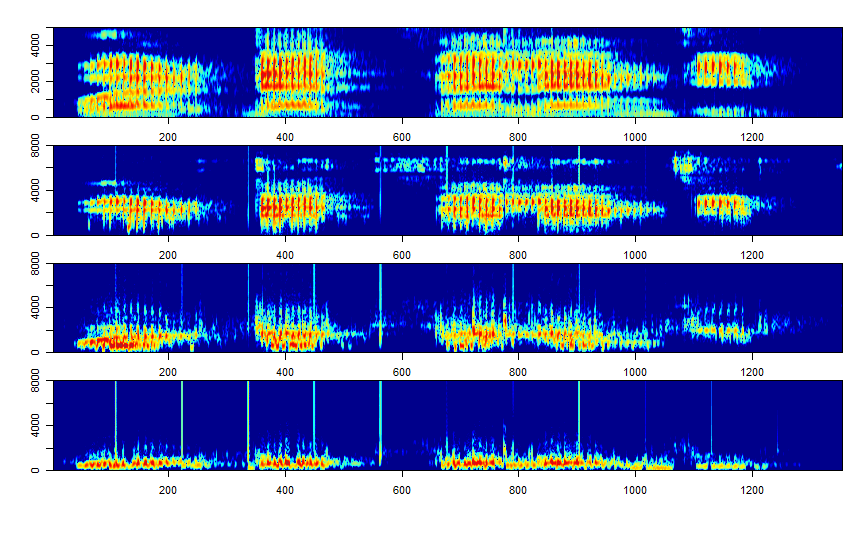
\includegraphics[width=\linewidth]{spectro_speak3_bis.png}
%  \caption{1b}
  \label{fig:sfig2}
\end{subfigure}\\
\begin{subfigure}{0.8\textwidth}
  \centering
  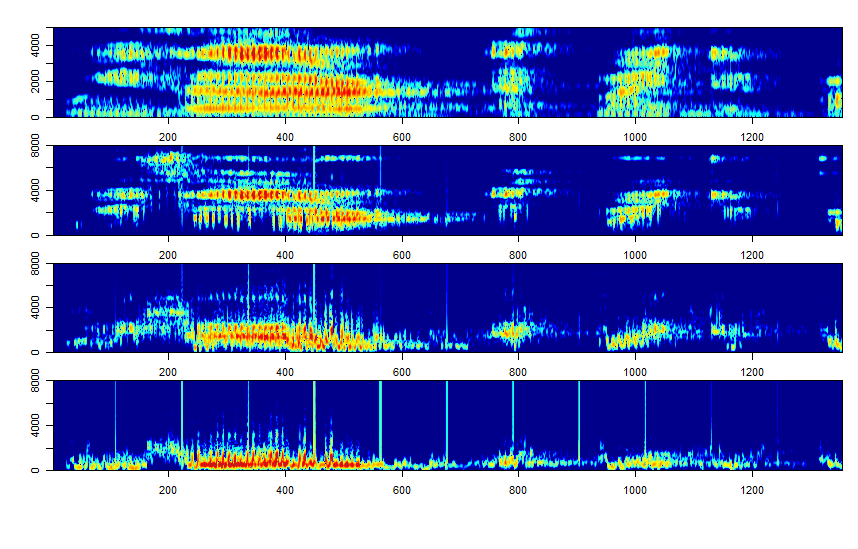
\includegraphics[width=\linewidth]{spectro_speak3_tris.png}
%  \caption{1b}
  \label{fig:sfig2}
\end{subfigure}
\label{fig1}
\caption{Spectrograms of three sentences for speaker 1 (male voice). From the top: the original signal, IMF1, IMF2 and IMF3 respectively.}
\end{figure}
\end{landscape}









\end{document}